\documentclass[english]{article}

%% Packages pull in extra commands:
%% http://en.wikibooks.org/wiki/LaTeX/Packages

\usepackage{hyperref}
\usepackage[latin9]{inputenc}
\usepackage[letterpaper]{geometry}
\geometry{verbose,tmargin=1in,bmargin=1in,lmargin=1in,rmargin=1in}
\usepackage{amsmath}
\usepackage{amssymb}
\usepackage{graphicx}
\usepackage{float}
\usepackage{array}
\usepackage{enumerate}
\usepackage{tikz}

% New commands serve as shorthand for frequently used command combinations.
\newcommand{\ind}[1]{\mathbf{1}\left(#1\right)}
\newcommand{\bx}{\mathbf{x}}
\newcommand{\E}{\mathbf{E}}

\title{Fly By Logic - GUI User Manual}

\begin{document}

\maketitle

\section{User Interface}
\begin{enumerate}
    \item 
        \begin{figure}[H]
        \centering
        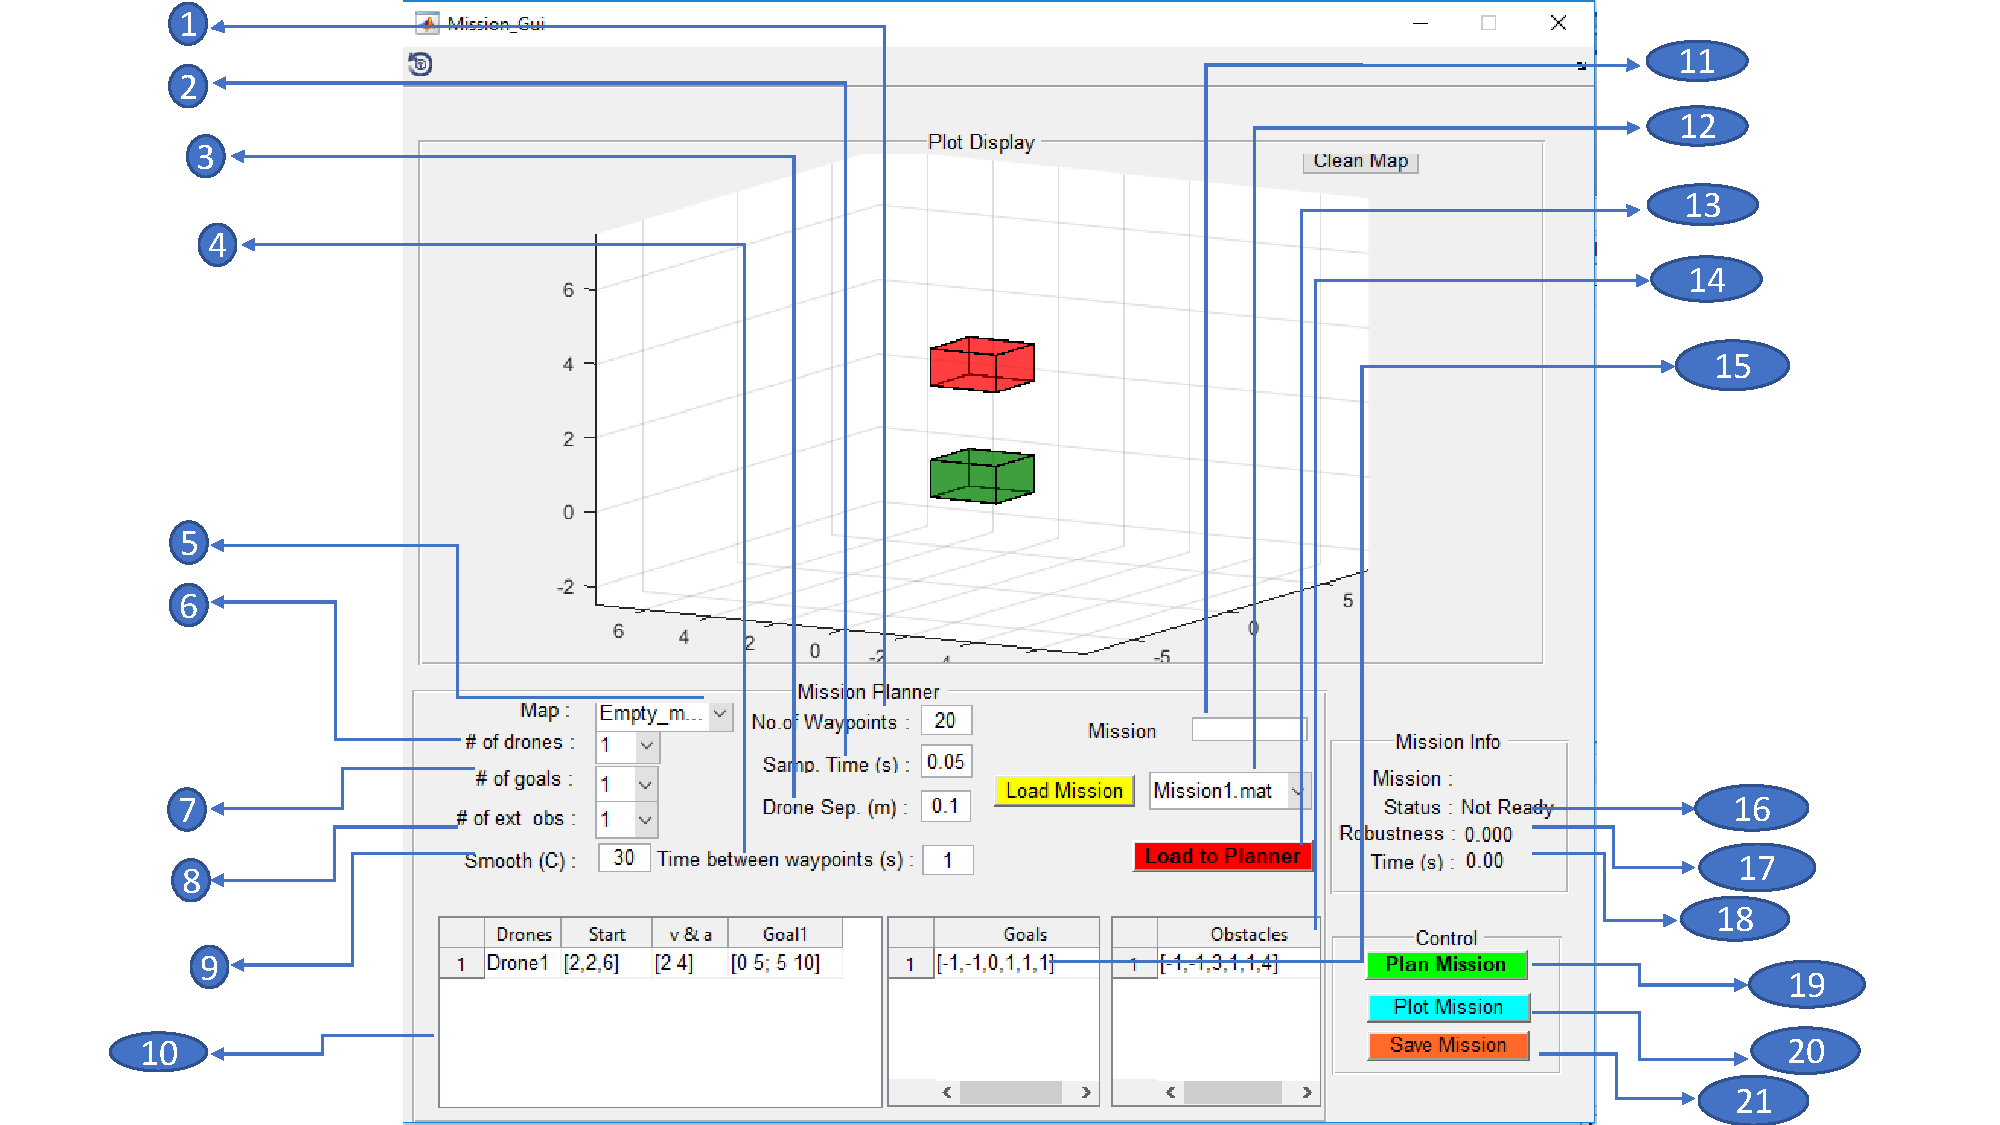
\includegraphics[scale=0.6]{layout.pdf}
    \end{figure}
\end{enumerate}
\section{GUI Nomenclature}
\item With reference to the indexing on the GUI Layout, each feature is explained below
\begin{enumerate}
    \item \textbf{No. of Waypoints} - Given the start and goal positions, the planner generates waypoints between these two. And this parameter denotes the number of high samples waypoints to be generated between each two waypoints given by the planner.
    \item \textbf{Samp. Time (s)} - Abbreviated to Sampling Time. This depicts the rate at which the high sampled points are generated.
    \item \textbf{Drone Sep. (m)} - The minimum distance that the drones to be maintained between each other.
    \item \textbf{Time between waypoints (s)} - The time taken by the drone to travel between any two way points generated by the planner.
    \item \textbf{Map} - Loads the Map. These maps can be designed and saved by the user to load to the planner.
    \item \textbf{$\#$ of drones} - Number of drones required to perform a specific mission.
    \begin{figure}[H]
        \centering
        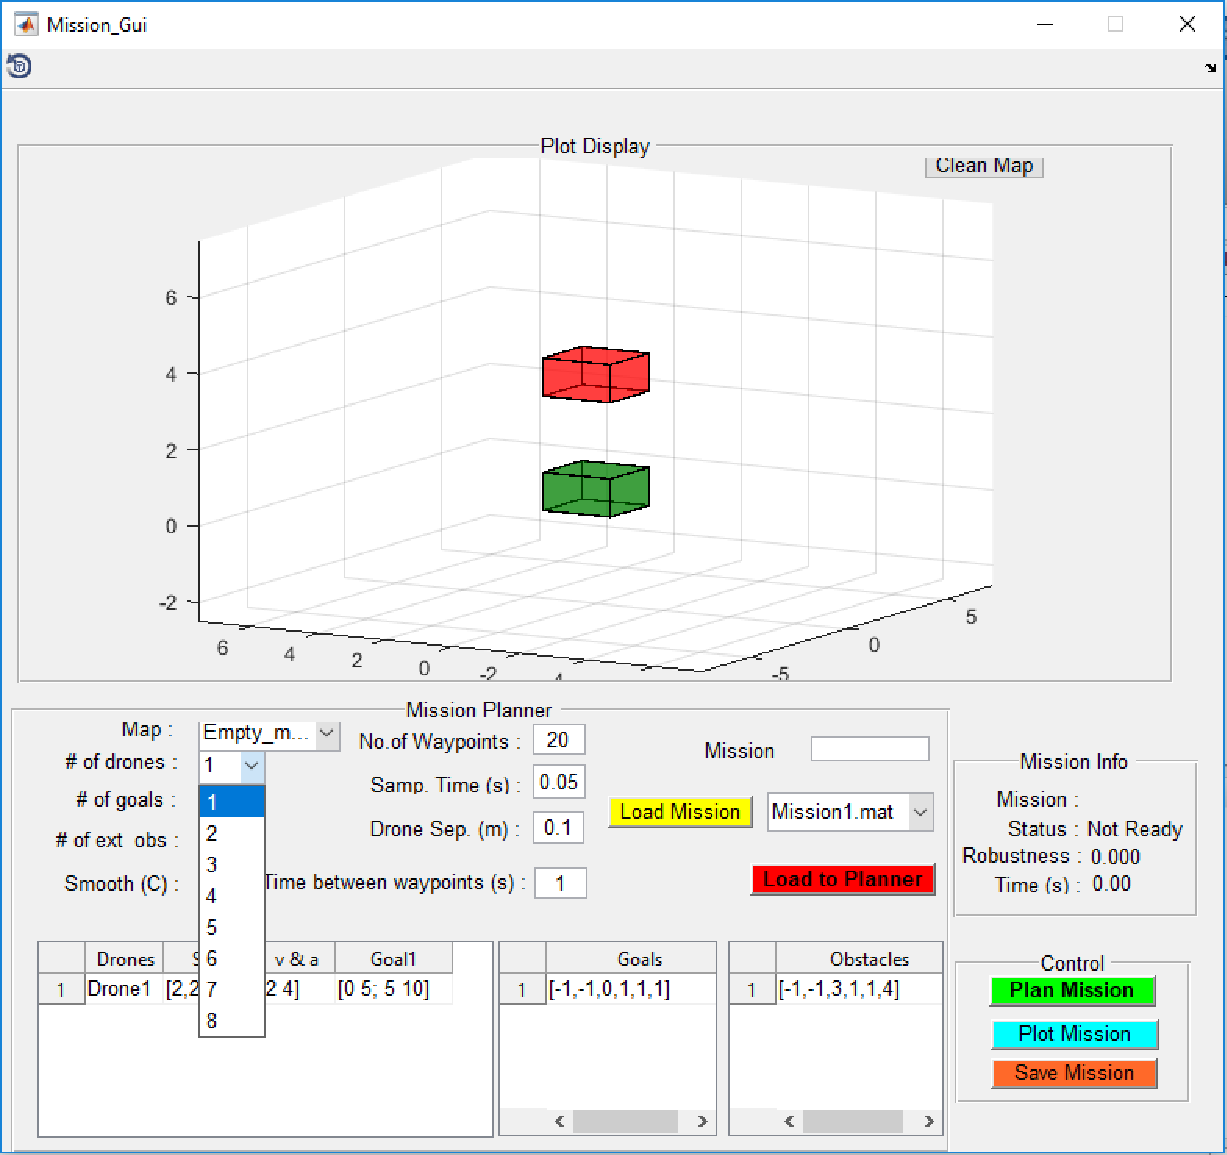
\includegraphics[scale=0.5]{drones.pdf}
    \end{figure}
    \item \textbf{$\#$ of goals} - Number of goal sets for the drones to oblige in the given time interval for a specific mission.
    \begin{figure}[H]
        \centering
        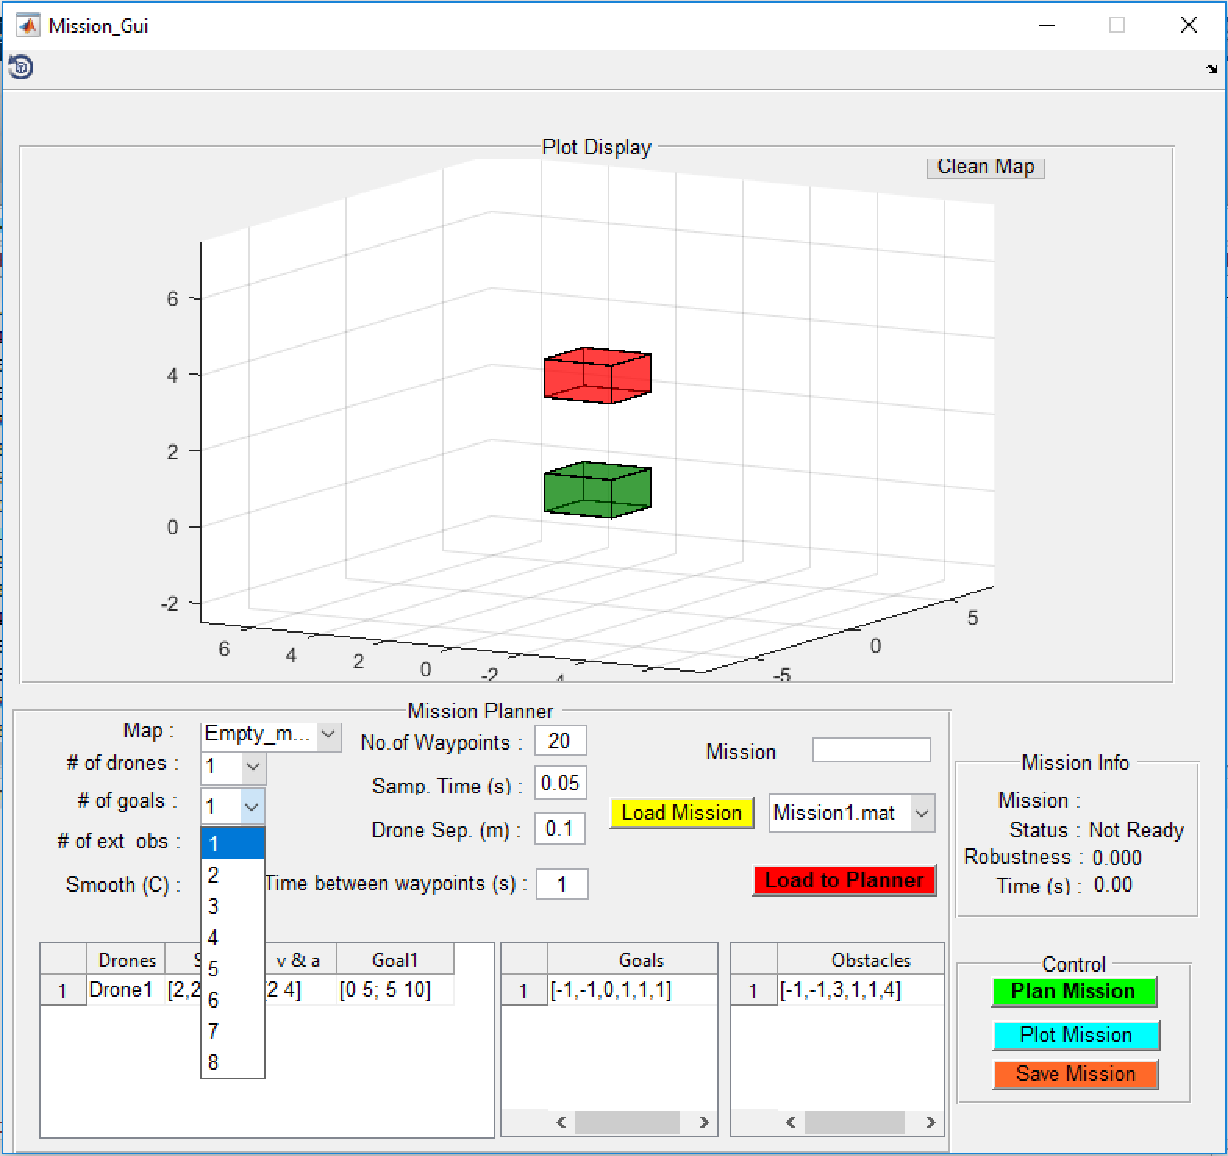
\includegraphics[scale=0.4]{goals.pdf}
    \end{figure}
    \item \textbf{$\#$ of ext obs} - Number of external obstacles that the drones need to avoid while executing the mission.
    \begin{figure}[H]
        \centering
        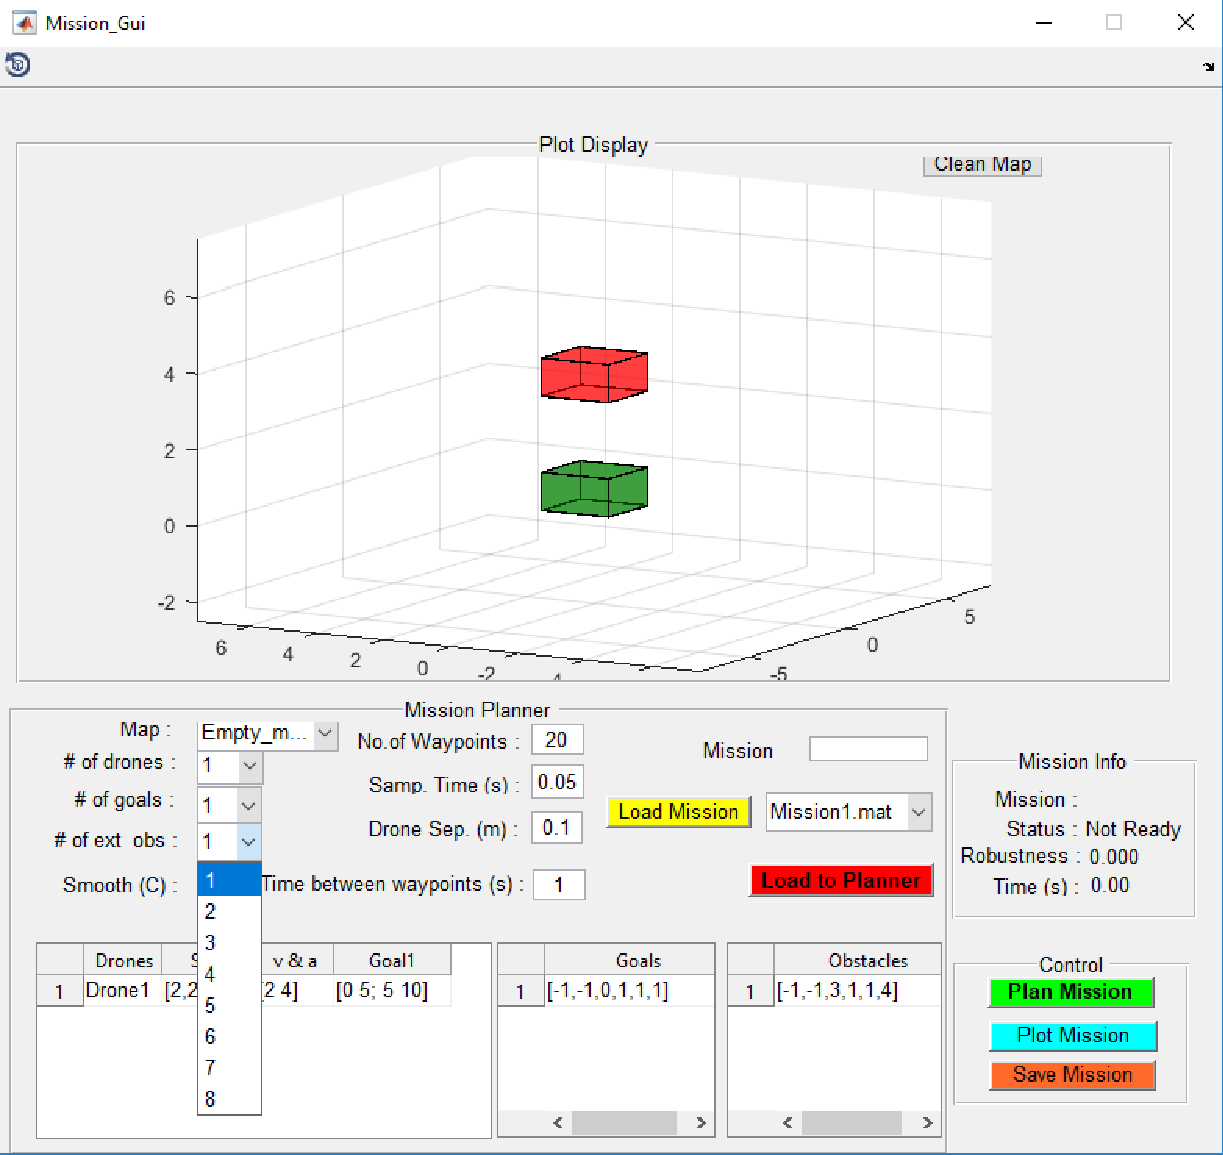
\includegraphics[scale=0.5]{obs.pdf}
    \end{figure}
    \item \textbf{Smooth (C)} - Smoothing parameter that is used to smooth the robustness function to solve the optimization problem.
    \item \textbf{Mission Table} - This table gives the core Mission parameters. It has three + n columns where n is the number of Goal time intervals. The first three columns of the table are \textbf{Drones}, \textbf{Start}, \textbf{v$\And$a}. The Drones column shows the Drone number. The Start column gives the 3D Cartesian of the start position of the respective drone. This should be in the format \textbf{[x,y,z]}. The v$\And$a column gives the velocity and acceleration bounds on the respective drone. This should be in the format \textbf{[v,a]}. v is in $\frac{m}{s}$ and a is in $\frac{m}{s^2}$ . The rows indicate these parameter with respect to \textbf{$\#$ of drones}\\
    The rest of the n columns gives the Goal time intervals that the respective drone need to obey for a specific mission. n is equal to the \textbf{$\#$ of goals} parameter. The format for the goal time interval is an array \textbf{[$t_1 t_2; t_3 t_4$]}. Consider an example where the goal time interval is [0 5; 10 15] and there is one goal. This says that, the respective drone should reach the goal set eventually in [0 5] time interval and it should reach goal set again in [10 15] time interval. All the numbers in the goal time interval are in seconds. 
    \item \textbf{Mission} - Name of the custom mission to be saved. Custom missions are the missions designed by the user to be used in future.
    \item \textbf{Load Mission} - This enables user to load the previous missions that are saved by the user. 
    \begin{figure}[H]
        \centering
        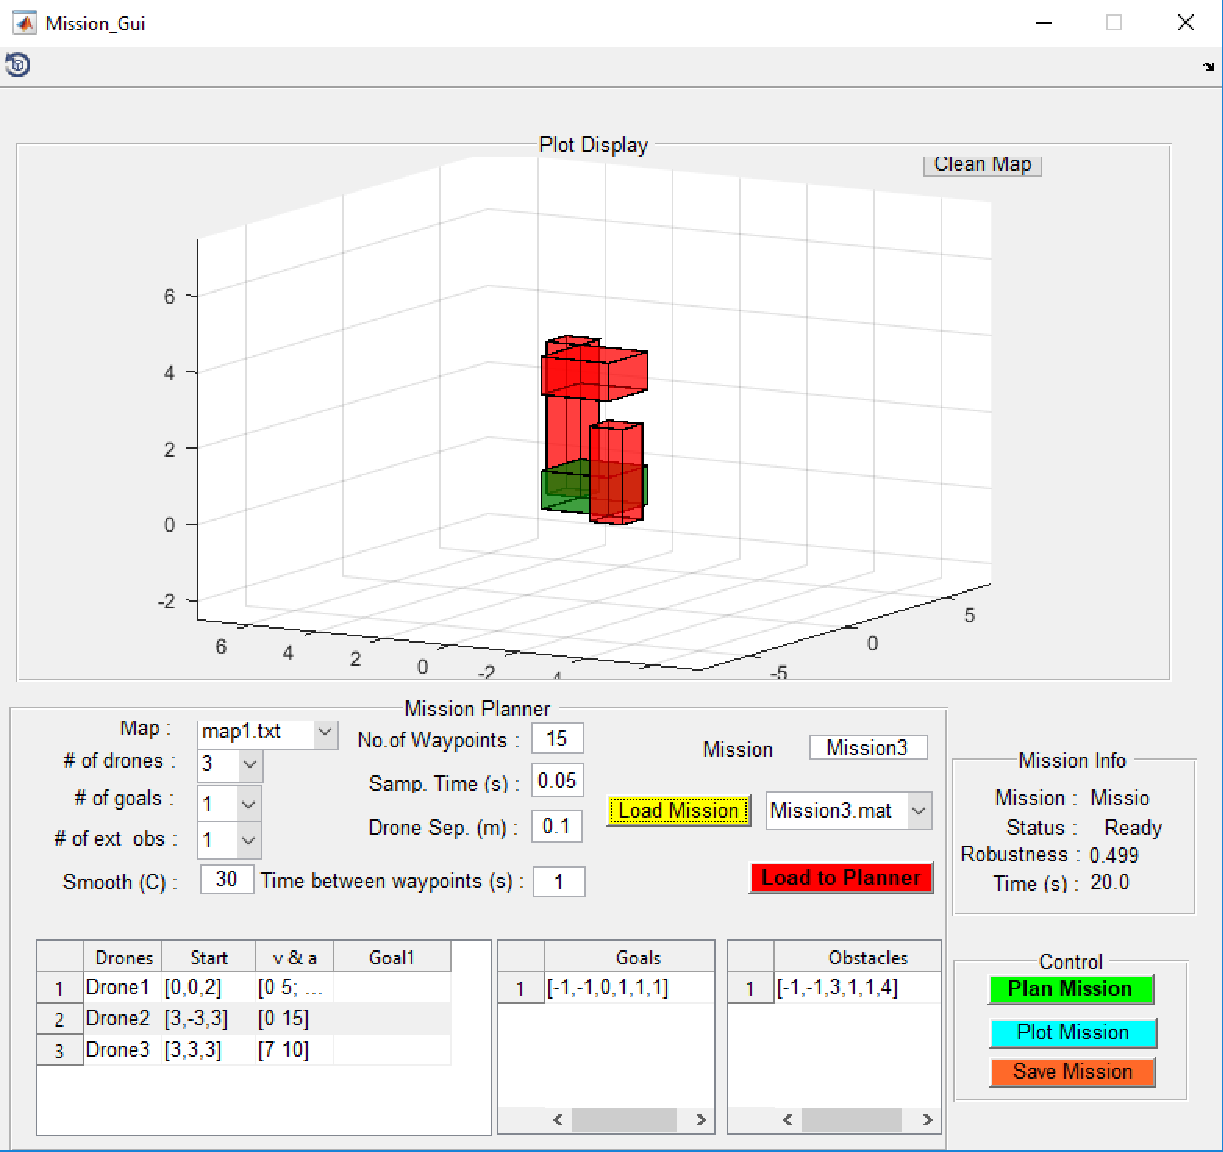
\includegraphics[scale=0.5]{load.pdf}
    \end{figure}
    \item \textbf{Load to Planner} - \textbf{TO BE WRITTEN}
    \item \textbf{Obstacles} - This table gives the Lower and Upper bounds of the x, y, z coordinates of the obstacles. The number of obstacles are decided by the \textbf{$\#$ of ext obs} parameter. Consider an example where the obstacle is denoted by [-1,-1,3,1,1,4]. This says that the Lower bound on x-coordinate is -1 and the Upper bound on x-coordinate is 1. Similarly, the Lower bound on y-coordinate is -1, the Upper bound on y-coordinate is 1 and Lower bound on z-coordinate is 3 and the Upper bound on z-coordinate is 4. This gives the shape of the obstacle to be a cuboid.
    \item \textbf{Goals} - This table gives the Lower and Upper bounds of the x, y, z coordinates of the Goals. The number of Goals by the \textbf{$\#$ of goals} parameter. Consider an example where the obstacle is denoted by [-1,-1,0,1,1,1]. This says that the Lower bound on x-coordinate is -1 and the Upper bound on x-coordinate is 1. Similarly, the Lower bound on y-coordinate is -1, the Upper bound on y-coordinate is 1 and Lower bound on z-coordinate is 0 and the Upper bound on z-coordinate is 1. This gives the shape of the Goal to be a cuboid.
    \item \textbf{Status} - This lets the user know if the mission is \textbf{Ready} to be planned. If the user loads one of the saved missions, this parameter lets the user know that the mission is \textbf{Ready} to be planned after the loading has completed. Else, this parameter shows \textbf{Not Ready}
    \item \textbf{Robustness} - This gives the robustness value of the mission after solving the optimization problem which is obtained by Planning the Mission through \textbf{Plan Mission} button. 
    \item \textbf{Time} Time taken to plan the mission.
    \item \textbf{Plan Mission} - This button lets the user decide to plan the mission once all the parameters to the mission are given to the GUI. 
    \item \textbf{Plot Mission} - This button lets the user to plot the mission once the mission has been planned.
    \item \textbf{Save Mission} - This button lets the user save the mission which is custom designed by the user. The user can choose to save the mission on a file name which can be given as an input in \textbf{Mission} parameter of the GUI.
\end{enumerate}
\section{Example Mission with Parameters}
\begin{figure}[H]
        \centering
        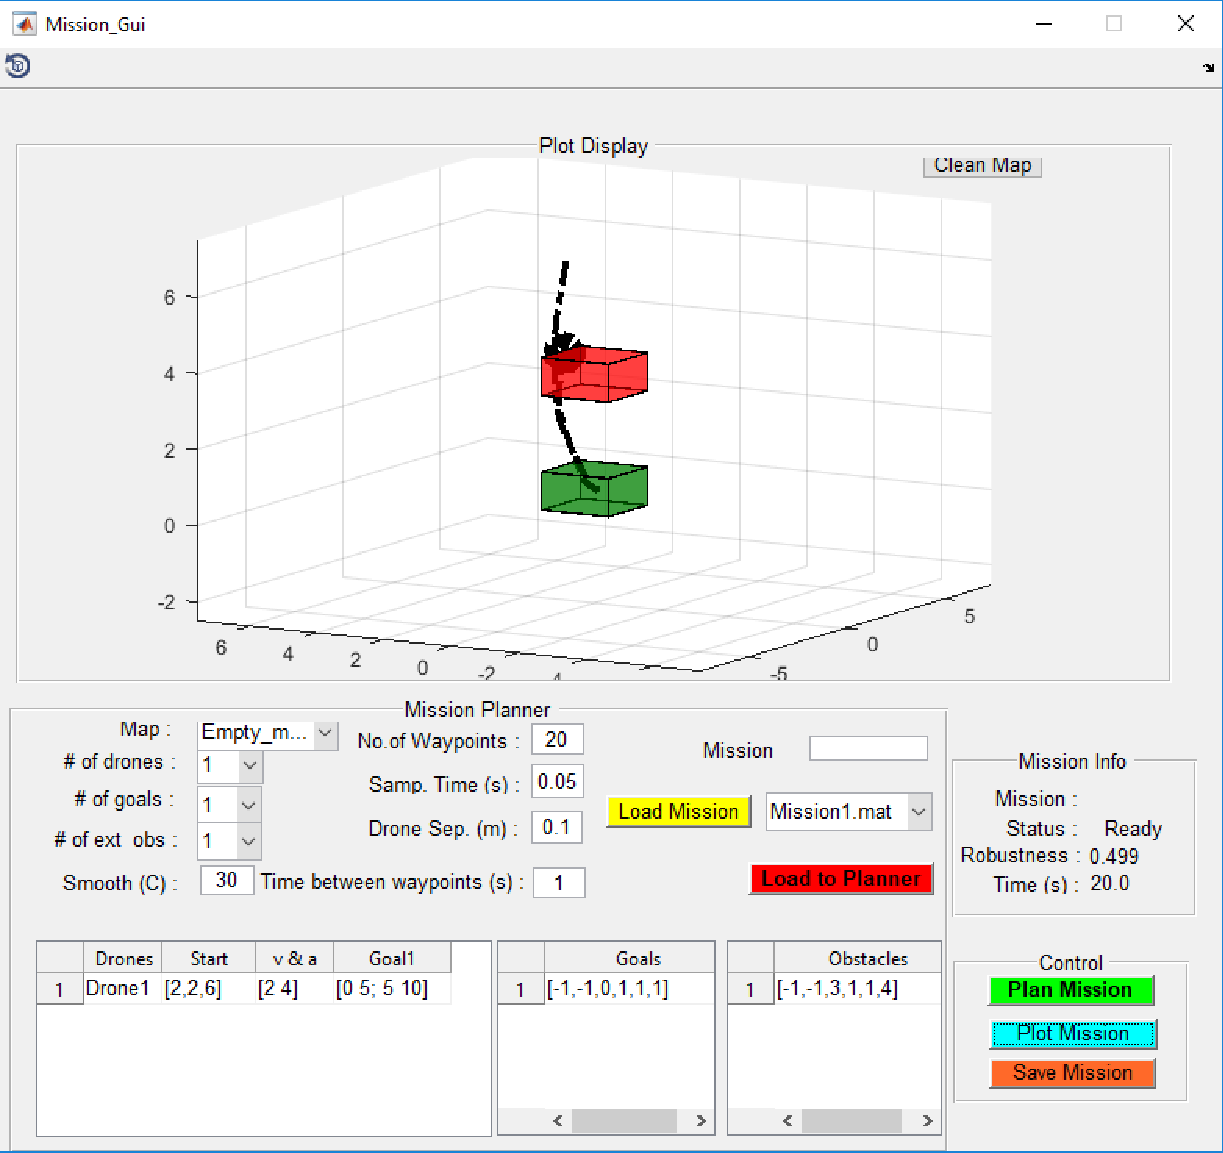
\includegraphics[scale=0.6]{example.pdf}
    \end{figure}
\end{document}
